\subsection{Datenbankdesign und Strukturkonzeption}
\label{subsec:datenbankdesign-und-strukturkonzeption}

In diesem Unterkapitel soll der Verlauf der Erstellung der Datenbank beschrieben und nachvollzogen werden. Es wurde in
den Anforderungen festgelegt, dass MariaDB zu erstellen genutzt werden soll. MariaDB ist ein kostenloses, relationales
Open-Source-Datenbankmanagementsystem, das aus einer Abspaltung von MySQL entwickelt wurde. MySQLs früherer
Hauptentwickler Michael Widenius hat das Projekt ins Leben gerufen.

Betrachtung der Anforderungen

Für das genaue Interpretieren und Umsetzen der Anforderungen wurde festgelegt, dass die Ersteller/-in der Datenbank erst
ein Konzept nach den festgelegten Anforderungen erarbeiten und umsetzen. Diese Umsetzung wird dann im Laufe der weiteren
Erstellung der Applikation, falls nötig, angepasst.

Konzeptionelles Datenmodell

Für das Erstellen der Konzeption des Datenbankmodelles wurde die XML-Struktur analysiert, um die Kenntnisse und Muster
aus Unterkapitel \ref{XML-Schema} abzuleiten.
Aus diesen Erkenntnissen wurde dann ein ER-Modell erstellt, siehe Abbildung \ref{fig: ER-Modell Überlegung der Datenbankstruktur}.
Im Folgenden wird das ER-Modell beschrieben.

Durch das Durchführen eines Testes wird ein Bericht erstellt. Dieser Bericht enthält einige Attribute, welche
Testinformationen, darunter die Seriennummern, das Datum und die Uhrzeit des Tests, die Materialnummer (DUT-ID), die
Konfigurations-Version und die Carrier-Bezeichnung enthalten. Zudem besitzt der Bericht eine Unterentität
Testbenchinformationen“, die die Hard- und Softwareversionen des Teststandes enthält. In der Unterentität Testmodelle
befinden sich Versions-, Zeit- und Ergebnisinformationen sowie drei Datensätze, welche die Testparameter und die Messdaten
enthalten. Diese Datensätze können den Phasen des Stromnetzes des Teststandes und somit den DUTs zugeordnet werden.
Zusätzlich zu dem Aufbau wurden hier schon Schlüsselattribute hinzugefügt, die später die primären Schlüssel der
Datenbanktabellen dienen sollen, orange markiert. Die Attribute sind hier nicht genau nach dem Inhalt der XML-Dateien
benannt aber an ihre genauen Bezeichnungen angelehnt.

\begin{figure}[H]
    \centering
    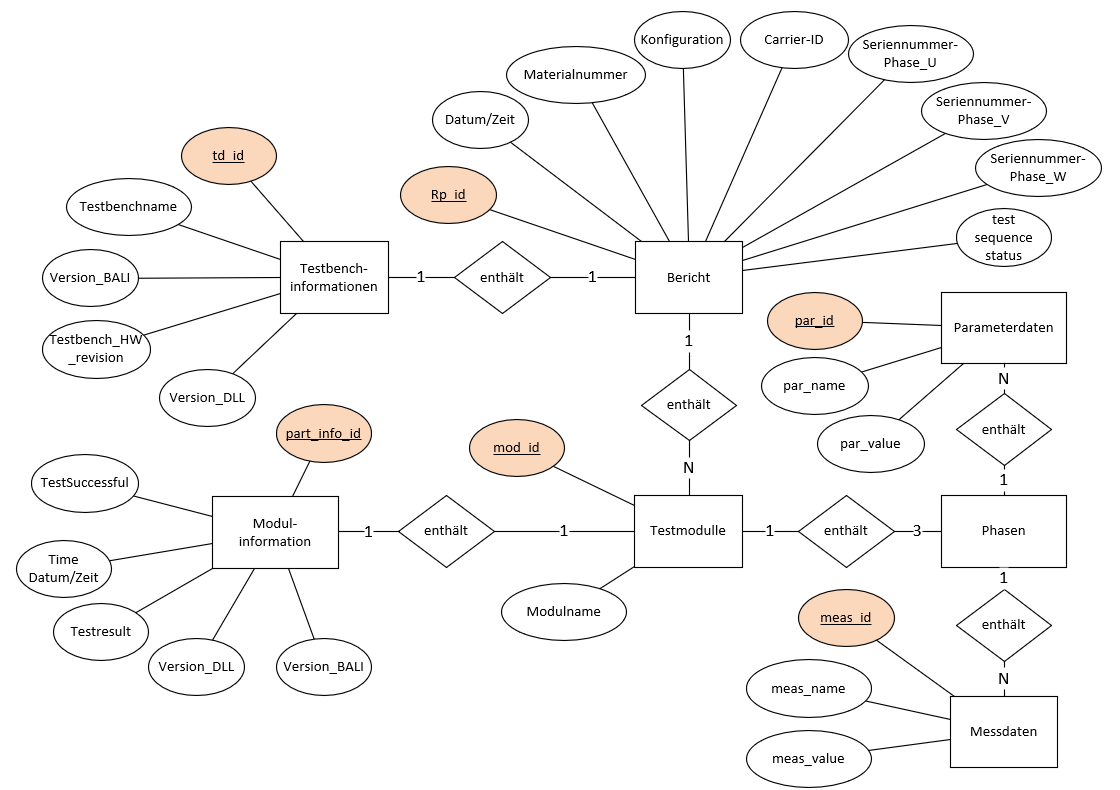
\includegraphics[width=0.95\textwidth]{Grafiken/Bild von ER-Modell}
    \caption{ER-Modell Überlegung der Datenbankstruktur}
    \label{fig: ER-Modell Überlegung der Datenbankstruktur}
    {Quelle: Eigene Darstellung mit Microsoft Visio}
\end{figure}

Aus diesem ER-Model wurde die Datenbanktabelle und ihre Verbindungen über Fremdschlüssel abgeleitet. In Abbildung \ref{ }
werden die Datenbanktabellen, ihre genauen Namensbezeichnungen der Tabelle und ihr Inhalt sowie ihre Verbindungen abgebildet.

